\chap{Geometría del frente de infección}{rugosidad}
\graphicspath{{figs/cap6}}


En este capítulo exploramos en profundidad las propiedades microscópicas del frente de infección, buscando describir la dinámica fundamental y universal del mismo. Nuevamente, estaremos resolviendo el sistema del modelo SIR espacial heterogéneo propuesto en el capítulo \ref{cap:SIR}. Es decir, el sistema
\begin{align}
    \partial_t S &=-\beta_{\vb r} SI + D_{S} \laplacian{S},\label{Seqdif}\\[.3cm]
    \partial_t I &=\beta_{\vb r} SI - \gamma I + D_{I} \laplacian{I},\label{Ieqdif}
\end{align}
con $(x,y) \in [0,L_x]\times[0,L_y]$ y condiciones iniciales
\begin{align*}
    I(x,y,0) &= 
    \begin{cases}
    I_0 & \text{si} \; (x,y) \in \Omega_0 \\
    0 & \text{si} \; (x,y) \notin \Omega_0  
    \end{cases}
    & ;&&
    S(x,y,0) &=
    \begin{cases}
    1-I_0 & \text{si} \; (x,y) \in \Omega_0 \\
    S_0 & \text{si} \; (x,y) \notin \Omega_0.
    \end{cases}
\end{align*}
donde $\Omega_0 = (0,\delta x) \times [0,Ly]$, es decir, la condición inicial consiste en un frente de infección plano. En cuanto a las condiciones de contorno tomamos condiciones periódicas en la dirección $y$ y condiciones de Dirichlet en la dirección $x$ dadas por
\begin{align*}
    I(0,y,t)=I(L_x,y,t)=S(0,y,t)=S(L_x,y,t)=0.
\end{align*}

Esta vez nos centraremos únicamente en obtener resultados sobre el medio DA. El tamaño de los sistemas utilizado para algunos resultados de este capítulo alcanzó $(L_x = 2^{16}, L_y =2^{11})$. Esto fue necesario para lograr alcanzar el tiempo de saturación $t_x$ del campo de desplazamiento del frente de infección.

En lo que sigue mostraremos resultados del ancho $\omega(L,t)$ y el factor de estructura $S(q,t)$ de la interfase. A partir de lo cual intentaremos determinar la clase de universalidad que la describe. Por otro lado, mostramos que una potencial ecuación de evolución para el campo de desplazamiento debe tener un término no lineal de tipo $(\nabla u)^2$, que concuerda con la clase de universalidad encontrada.


\sect{Ancho del frente de infección}{ancho}

\ssect{Diferencias por definición del campo de desplazamiento}{dif}

Comenzamos por estudiar el ancho del campo de desplazamiento $u(y,t)$ que define la interfase del frente de infección. Recordemos que el ancho $\omega(L_y,t)$, dado $u(y,t)$, es 
\begin{equation}
    \omega^2(L_y,t) = \langle (u(y,t) - u_{cm}(t))^2 \rangle_y, 
\end{equation} 
donde $u_{cm}(t) = \langle u(y,t) \rangle_y$ y $\langle \hdots \rangle_y$ toma la media espacial sobre la coordenada $y$. En el capítulo anterior utilizamos como campo de desplazamiento, que llamaremos ahora $u_0(y,t)$, a las posiciones $x$ que maximizan $I(x,y,t)$ dados $y$ y $t$, es decir,
\begin{equation}
    \max_x[I(x, y, t)]=I(u_0(y, t), y, t)
\end{equation}
En este capítulo, tendremos en consideración además una definición alternativa para el campo de desplazamiento, dada por 
\begin{equation}
    u_1(y,t) =  \frac{\int_{0}^{L_x} x \; I(x,y,t)}{\int_{0}^{L_x} I(x,y,t)}. 
\end{equation}
La diferencia fundamental entre estas definiciones, es que en un espacio discretizado el campo $u_0(y,t)$ está limitado a tomar los valores de la discretización en $x$. En cambio, el campo $u_1(y,t)$ es continuo y puede tomar cualquier valor entre $0$ y $L_x$. A continuación veremos que hay ciertas diferencias entre los resultados obtenidos con cada una de estas definiciones y que se deben tener en cuenta algunas sutilezas para que los resultados obtenidos sean consistentes entre sí.

Obsérvese la figura \ref{fig:omegas}, donde mostramos los resultados del ancho de la interfase con las distintas definiciones del campo de desplazamiento, $u_0(y,t)$ y $u_1(y,t)$, sobre un sistema de $L_x = 2^{16} \times L_y = 2^{11}$. Se realizaron 150 realizaciones utilizando un medio DA con $p=0.15$, $\beta = 1$ , $\gamma = 0.2$, $D_S = 0$ y $D_I=1$. Denotamos por $\omega_0$ y $\omega_1$ los anchos de $u_0(y,t)$ y $u_1(y,t)$, respectivamente. Recordemos también que $\overline{\cdots}$ denota promedio sobre realizaciones. Se observa que el ancho de la interfase, en ambos casos, crece siguiendo una ley de potencias con el tiempo hasta llegar a un valor de saturación, a partir del cual ya no crece más. Sin embargo, es claro que las curvas de $\overline{\omega_0}$ y $\overline{\omega_1}$ difieren notablemente, de hecho se observa que la pendiente en log-log es distinta, de modo que se podría pensar que la rugosidad del frente evoluciona con exponentes de crecimiento $\alpha/z$ distintos dependiendo de la definición que utilicemos para la interfase. Lo que realmente está sucediendo es que no estamos teniendo en cuenta el ancho intrínseco $\omega_i$ \cite{barabasi} asociado a la definición de $u_0(y,t)$, que no es otro que la discretización del espacio en $x$, igual a la unidad en este caso, es decir, $\omega_i = 1$. Si sustraemos $\omega_i$ de $\overline{\omega_0}$ obtenemos la curva $\overline{\omega}$ que es similar a la curva de $\overline{\omega_1}$ dentro del error. Esto muestra que para obtener los exponentes de universalidad que describen correctamente la interfase, es necesario tener en cuenta el ancho intrínseco al utilizar $u_0(y,t)$. 

Por otro lado, el hecho de que el ancho sature a un valor finito, recordando lo discutido en el capítulo \ref{cap:intro}, indica que hay una correlación entre puntos de la interfase, la cual se extiende lateralmente, caracterizada por una longitud de correlación $\xi_{||}(t)$ que crece hasta alcanzar el tamaño del sistema, momento en el cual satura el ancho de la interfase. Este fenómeno permite descartar una dinámica de tipo Poisson para la interfase, ya que en este caso el ancho de la interfase no satura.

Podríamos intentar obtener el exponente de crecimiento $\alpha/z$ que describe la ley de potencias con que crece el ancho $t^{\alpha/z}$ a partir de los resultados de la figura. Pero no es el método más aconsejable para determinar los exponentes de universalidad, dado que el ancho $\omega(L_y,t)$ es una cantidad integrada sobre todas las escalas, de modo que esto nos daría un exponente de crecimiento efectivo. Es más seguro obtener los exponentes de un observable como el factor de estructura, tal como haremos más adelante, que nos permite discriminar distintas escalas. Sin embargo, para no quedarnos con un solo método, a continuación determinamos los exponentes de rugosidad $\alpha$ y dinámicos $z$, utilizando los datos del ancho de la interfase con diferentes tamaños de sistema $L_y$.


\begin{figure}[t]
    \centering
    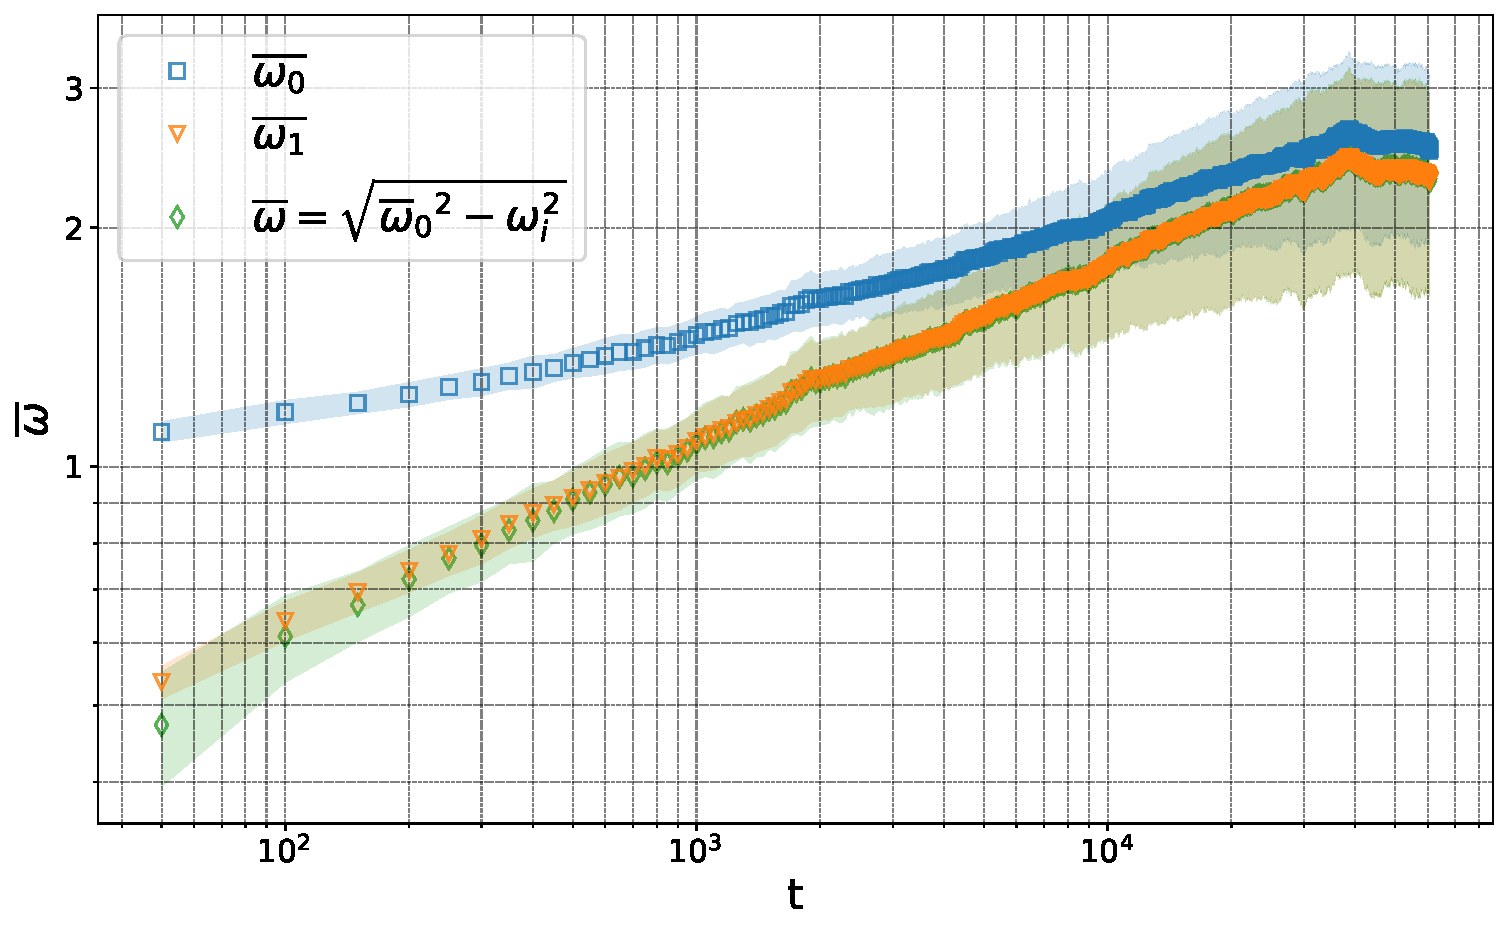
\includegraphics[width=\imsizeL]{omegas.pdf}
    \caption{Se muestran los promedios del ancho del campo de desplazamiento, $\overline{\omega_0}$ y $\overline{\omega_1}$, correspondientes a distintas definiciones del mismo, $u_0(u,t)$ y $u_1(y,t)$ respectivamente, sobre 150 simulaciones en un sistema de tamaño $L_x = 2^{16} \times L_y = 2^{11}$. Se observa que al sustraer el ancho intrínseco $\omega_i = 1$ de $\overline{\omega_0}$ se obtiene $\overline{\omega}$, una curva similar (dentro del error) a la de $\overline{\omega_1}$ que representa correctamente la dinámica del crecimiento rugoso. Se utilizaron los parámetros $\beta = 1$, $\gamma = 0.2$, $D_I = 1$, $D_S = 0$ y $p=0.15$.}  
    \label{fig:omegas}
\end{figure}


\ssect{Exponente de rugosidad y dinámico}{z_alpha}

\begin{figure}[!b]
    \centering
    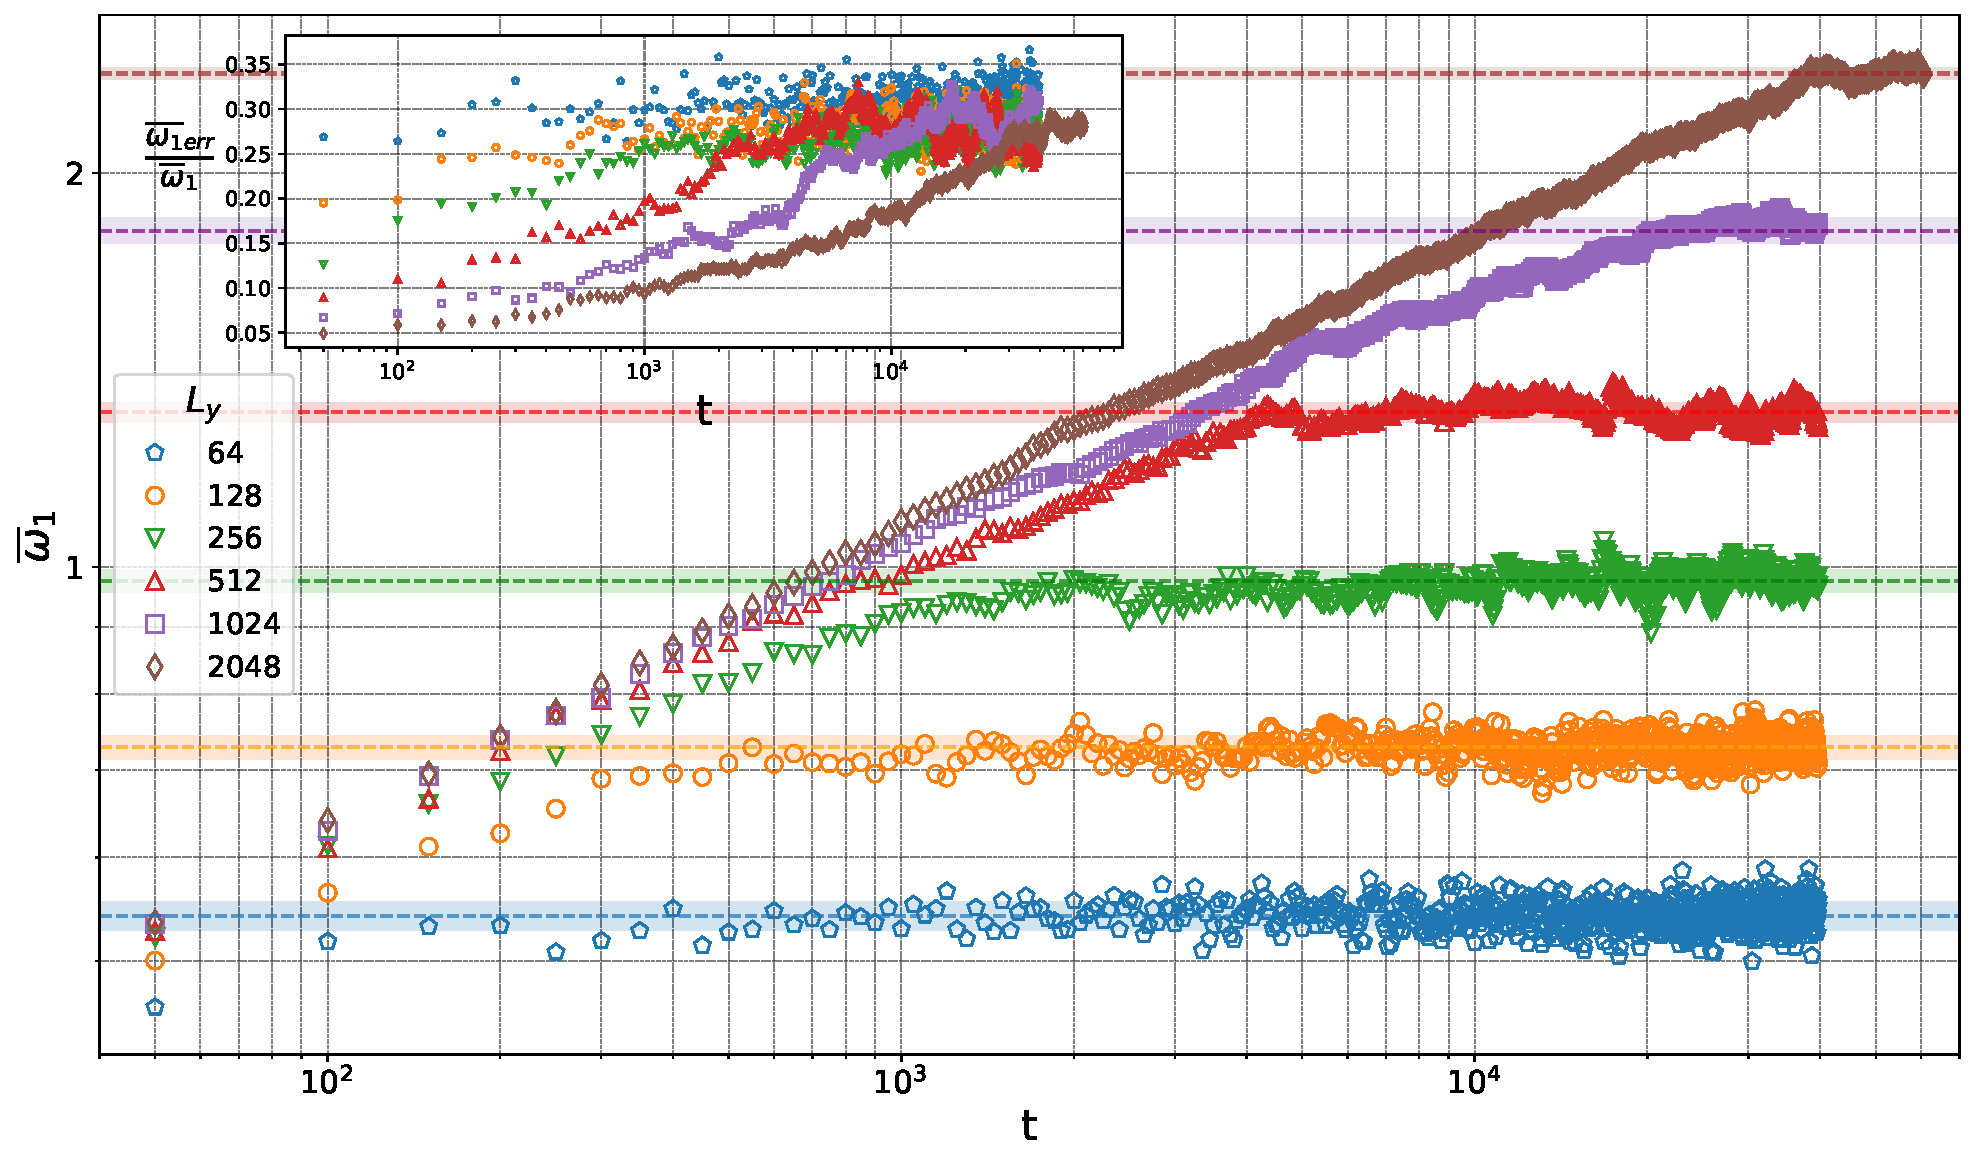
\includegraphics[width=\imsizeL]{omega1_Ls.pdf}
    \caption{Ancho del frente $\overline{\omega_1}$ para diferentes tamaños $L_y$ del sistema con $L_x = 2^{16}$. Se observa que el ancho del frente sigue una ley de potencias hasta alcanzar un valor de saturación que se indica con línea a trazos horizontal (- - -) y varía con $L_y$. En el \textit{inset} se muestra el error relativo de cada curva. En sombras de colores se indican dos desviaciones estándar del valor de saturación del ancho para cada curva. Se promedió sobre 150 realizaciones de desorden. Se utilizaron los parámetros $\beta = 1$, $\gamma = 0.2$, $D_I = 1$, $D_S = 0$ y $p=0.15$.}
    \label{fig:omega1_Ls}
\end{figure}

Para determinar los exponentes de rugosidad y dinámico de la interfase, debemos recordar algunas leyes de potencias discutidas en el capítulo \ref{cap:intro}. Si $t_x$, el tiempo de saturación, es el tiempo en el cual el ancho de la interfase satura, entonces
\begin{equation}
    \omega(L_y,t \gg t_x) = \omega_{sat}(L_y) \propto L_y^{\alpha},
    \label{eq:omega_sat}
\end{equation}
donde $\alpha$ es el exponente de rugosidad de la interfase. Mientras que,
\begin{equation}
    t_x \propto L_y^z,
    \label{eq:t_x}
\end{equation}
donde $z$ es el exponente dinámico.

En la figura \ref{fig:omega1_Ls} se muestra $\overline{\omega}_1(L_y,t)$ para distintos tamaños de interfase $L_y$ con $L_x = 2^{16}$ fijo. El tamaño de $L_x$ se eligió así para alcanzar el tiempo de saturación $t_x$, dado que el mismo crece como $L^z_y$ lleva mucho tiempo de simulación en sistemas grandes y por lo tanto se necesita mucho espacio a recorrer en $x$ para alcanzarlo. Se determinó el ancho de saturación $\overline{\omega_{sat}(L_y)}$ para cada $L_y$, este se indica en línea a trazos horizontal en la figura \ref{fig:omega1_Ls}. Luego, determinamos los tiempos de saturación $t_x$ para cada $L_y$, se consideró como tal al mínimo valor de tiempo en el cual el ancho de la interfase se encuentra a menos de dos desviaciones estándar del valor de saturación $\omega_{sat}(L_y)$.

En las figuras \ref{fig:omega_txvsL}a y \ref{fig:omega_txvsL}b se muestran $\overline{\omega_{sat}}$ y $t_x$ respectivamente, como función de $L_y$. Se observan los ajustes de las leyes de potencia \ref{eq:omega_sat} y \ref{eq:t_x}, a partir de los cuales se determinó los exponentes de rugosidad y dinámico, los resultados se muestran en la tabla \ref{tab:exponentes}. 

El exponente de rugosidad $\alpha$ se calculó con $\overline{\omega}_0$, $\overline{\omega}_1$ y $\overline{\omega}$, se observa nuevamente cómo la curva asociada a $\overline{\omega}_0$ difiere de las curvas de $\overline{\omega}_1$ y $\overline{\omega}$ dando lugar a un exponente de rugosidad erróneo como consecuencia de no ignorar el ancho intrínseco. Sin embargo, esto no interfiera a la hora de obtener el exponente dinámico dado que no afecta al tiempo de saturación. Y tanto $\overline{\omega}_0$ como $\overline{\omega}_1$ dan exponentes similares.

\begin{figure}[!b]
    \hspace*{-1.5cm}
    \begin{subfigure}{.57\textwidth}
      \centering
      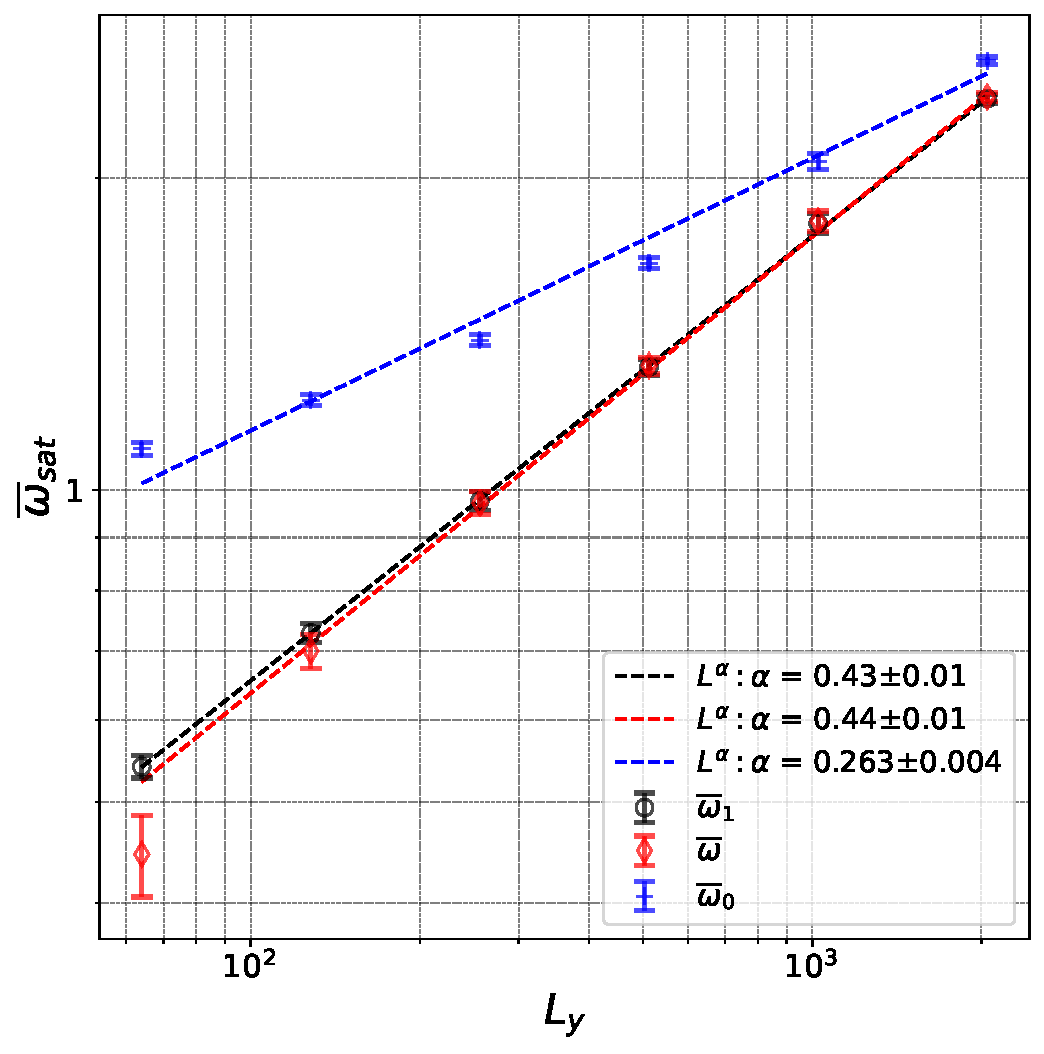
\includegraphics[width=1\textwidth]{omegavsL.pdf}
      \caption{}
    \end{subfigure}
    \begin{subfigure}{.57\textwidth}
      \centering
      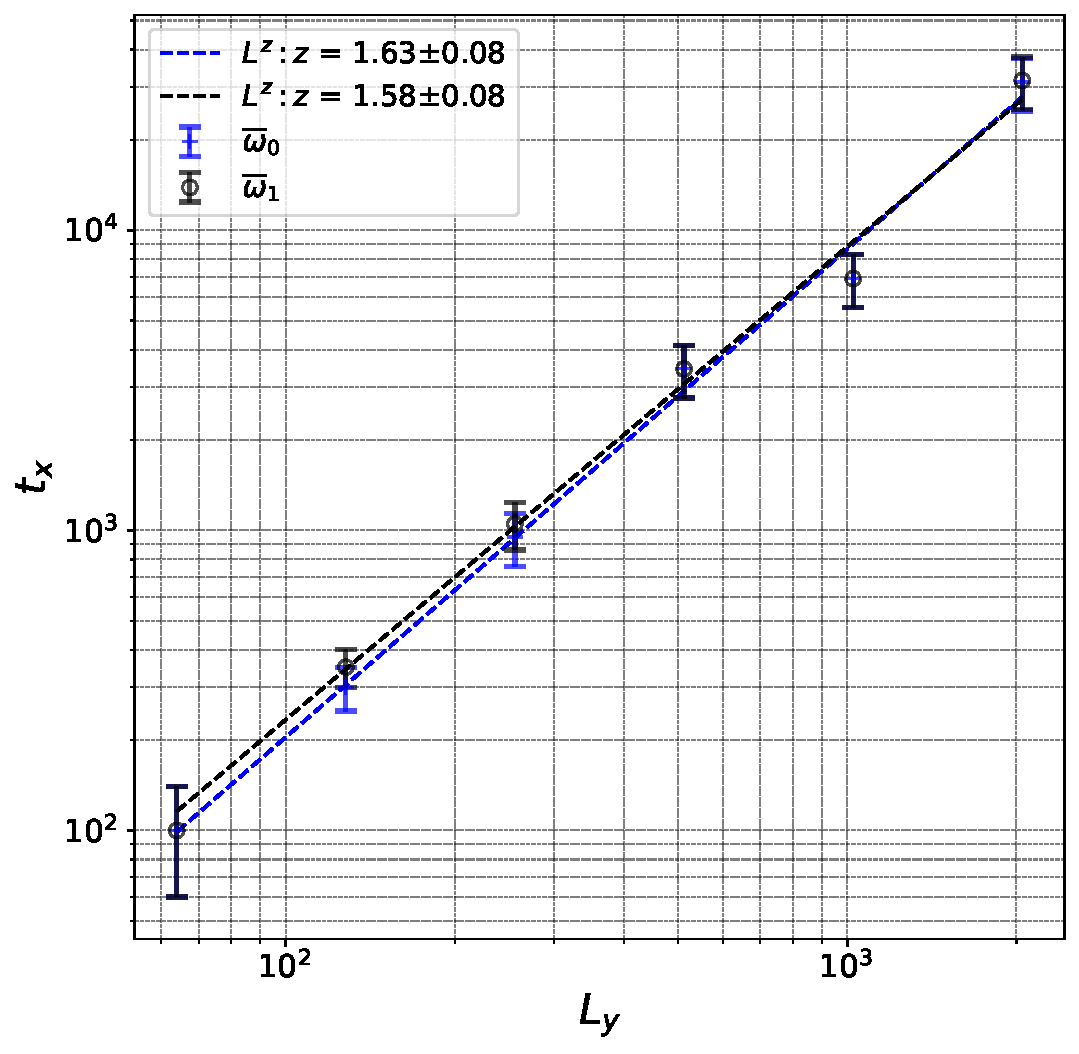
\includegraphics[width=1\textwidth]{txvsL.pdf}
      \caption{}
    \end{subfigure}
    \caption{\textbf{(a)}Ancho de saturación $\omega_{sat}$, usando $\overline{\omega}_0$, $\overline{\omega}_1$ y $\overline{\omega}$, en función del tamaño $L_y$ de la interfase. Se muestran los ajustes de potencia $L^\alpha$ con los que se determinó el exponente de rugosidad $\alpha$. \textbf{(b)} Tiempo de saturación $t_x$ del ancho de la interfase, $\overline{\omega}_0$ y $\overline{\omega}_1$, en función del tamaño $L_y$ de la interfase. Se muestran los ajustes de potencia $L_y^z$ con los que se determinó el exponente dinámico $z$.}
    \label{fig:omega_txvsL}
\end{figure}


De las clases de universalidad discutidas en el capítulo \ref{cap:intro} vemos que el exponente dinámico $z$ obtenido aquí únicamente concuerda con KPZ, $z = \frac{3}{2}$. Sin embargo, el exponente de rugosidad $\alpha\approx 0.42$ determinado no es el mismo que en KPZ, $\alpha = \frac{1}{2}$. Esto podría deberse a que quizás estamos subestimando los valores de saturación del ancho en los sistemas de mayor tamaño, como $L_y = 1024,2048$, y que quizás sea necesario llegar a un mayor tiempo de simulación para obtener estos valores más precisamente.

\begin{table}[t]
    \centering
    \begin{tabular}{@{}cccc@{}}
    \toprule
     & $\alpha$     & $z$    \\ \midrule
    $\overline{\omega}_0$     & $0.254\pm0.004$ & $1.58 \pm 0.08$ \\
    $\overline{\omega}_1$    & $0.42\pm0.01$ & $1.53 \pm 0.08$ \\
    $\overline{\omega}  $  & $0.43\pm0.01$ & - \\
    \end{tabular}
    \caption{Exponentes de rugosidad y dinámico obtenidos de los ajustes $\omega_{sat}(L_y) \propto L_y^{\alpha}$ y $t_x \propto L_y^z$ respectivamente, para distintas definiciones del ancho de la interfase.}
    \label{tab:exponentes}
\end{table}

En la figura \ref{fig:colapse} se muestra el colapso de $\overline{\omega}_1$ que se obtiene escaleando $\overline{\omega}_1$ por $L^\alpha$ y el tiempo $t$ por $L^z$. Para ello se utilizó los exponentes determinados previamente con $\overline{\omega}_1$. Se observa que el colapso es bueno, lo que indica que los exponentes determinados con estos datos son acertados.

En resumen, determinamos los exponentes de rugosidad $\alpha$ y dinámico $z$, y observamos que el exponente dinámico concuerda con el exponente dado por KPZ, aunque el exponente de rugosidad se encuentra subestimado. Sin embargo, la coincidencia del exponente dinámico nos motiva a pensar en la idea de que la dinámica del frente puede estar descrita por un término no lineal $(\nabla u)^2$ de tipo KPZ. A continuación intentaremos verificar esta hipótesis observando si hay alguna dependencia de la velocidad del frente con la inclinación del mismo.

\begin{figure}[!b]
    \centering
    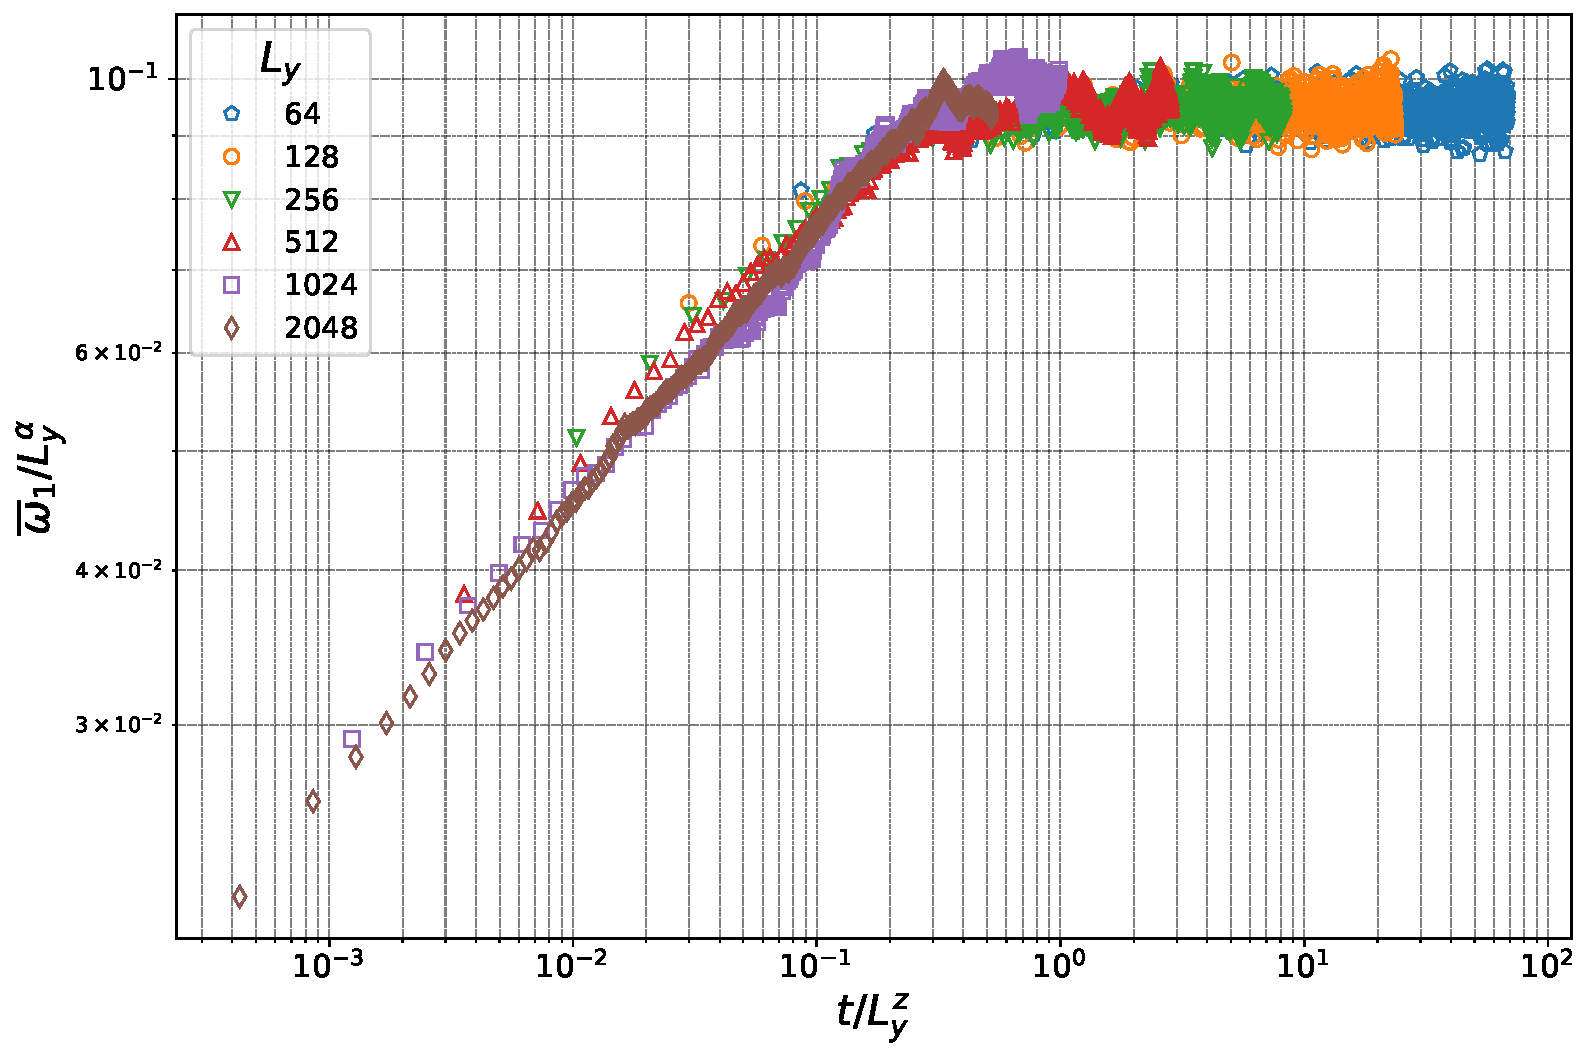
\includegraphics[width=\imsizeL]{colapse.pdf}
    \caption{Se muestra el colapso de las curvas para el ancho $\overline{\omega}_1$ al dividir por $L_y^{\alpha}$ y  escalear el tiempo por $L^z$.}
    \label{fig:colapse}
\end{figure}


\sect{Velocidad con frente inclinado}{vel}

Para verificar si la dinámica de la interfase presenta algún término no lineal debemos recordar nuevamente lo visto en el capítulo \ref{cap:intro} respecto a la velocidad de una interfase descrita por la ecuación de KPZ (ecuación \ref{KPZ}). Ahí vimos que la velocidad media de dicho frente depende del término no lineal de la siguiente manera (ecuación \ref{v_kpz}):
\begin{equation}
    v = v_0 + \frac{\lambda}{2L} \int_0^L d^d\mathbf{x} \overline{\left(\nabla h\right)^2}.
\end{equation}
Reemplazando por la notación que hemos estado utilizando para la velocidad del frente de infectados $c$ y el campo de desplazamiento $u(y,t)$, esto es,
\begin{equation}
    c = c_0 + \frac{\lambda}{2L_y} \int_0^{L_y} dy \overline{\left(\partial_y u\right)^2}.
    \label{c_m}
\end{equation}

De modo que podemos forzar la interfase a tener una inclinación determinada $m$ en la condición inicial, de manera tal que $\partial_y u \approx m$. Luego, al reemplazar esto en \ref{c_m}, obtenemos que la velocidad del frente depende cuadráticamente con la inclinación del mismo,
\begin{equation}
    c = c_0 + \frac{\lambda}{2} m^2.
\end{equation}

Recordemos que esto es así solo si existe un término no lineal que contribuye a la dinámica de la interfase. De otra manera, la velocidad del frente permanece inalterada ante una inclinación del mismo.

Para verificar esto alcanzó con trabajar con sistema ``chicos'' de $1024\times1024$, se utilizó un medio DA con $\gamma = 0.2$, $D_S = 0$,$D_I=1$, $p=0.15$ y distintos valores de $\beta$. En la figura \ref{fig:tilted_velocity}a se muestra la velocidad del frente en función de la inclinación inicial del mismo para distintos valores de $\beta$. Efectivamente, encontramos que la velocidad depende cuadráticamente con la pendiente del frente, lo que prueba la existencia de una componente no lineal en la dinámica del mismo.

Más aún, al realizar las simulaciones con distintos valores de $\beta$ pudimos determinar la constante de KPZ $\lambda$ ajustando las parábolas y encontramos que $\lambda$ es proporcional a la velocidad $c(0)$, de hecho $\lambda \approx c(0)$, tal como se muestra en la figura \ref{fig:tilted_velocity}b. Esto implica que el efecto que tiene el término no lineal, propio de KPZ, depende directamente de la velocidad del frente, cumpliéndose que $\lambda\to0$ cuando $c(0)\to0$, característico de la clase de universalidad de KPZ con origen cinético \cite{barabasi}. Esta podría ser otra razón por la cual el exponente de rugosidad $\alpha$ fue subestimado en la sección \ref{ssec:z_alpha}. 

\begin{figure}[h]
    \hspace*{-1cm}
\begin{subfigure}{0.55\textwidth}
    \centering
    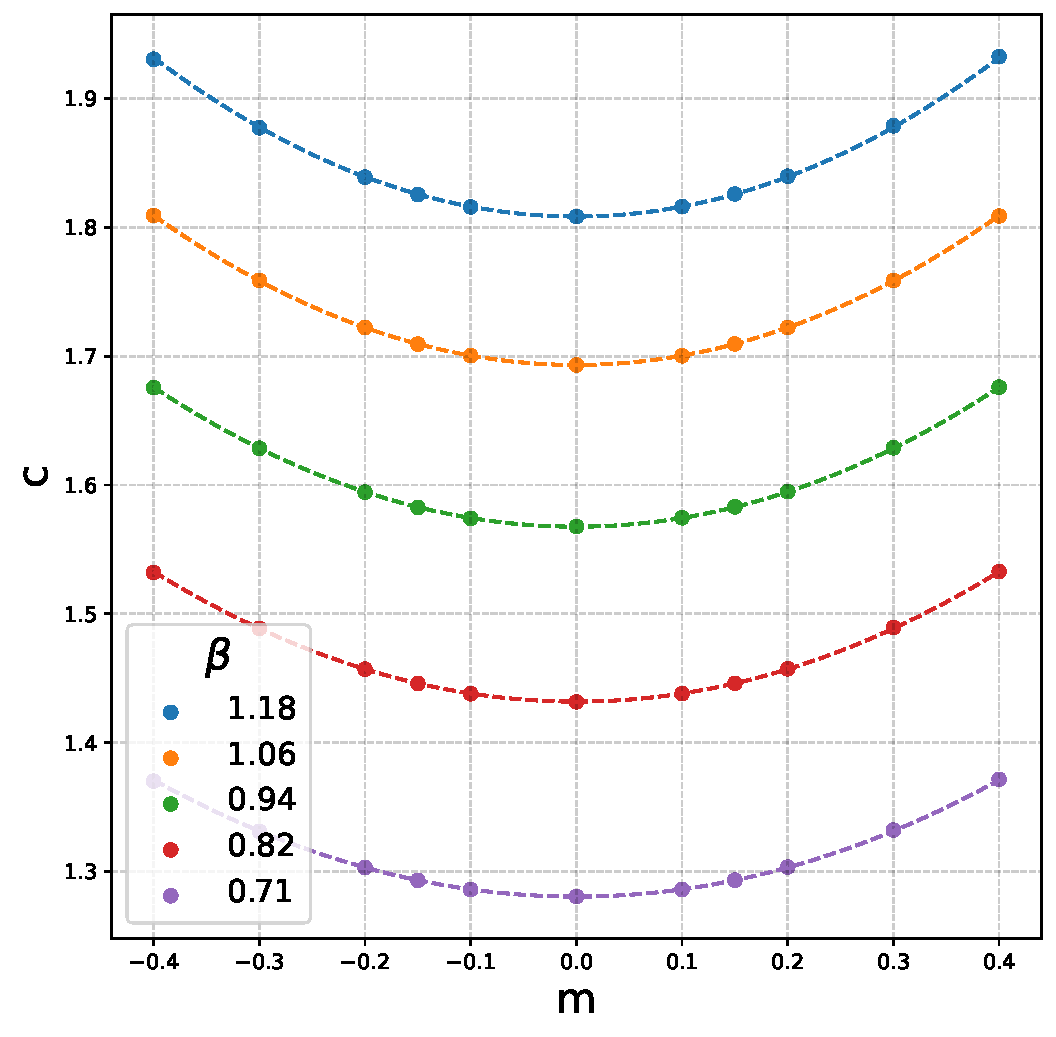
\includegraphics[width=\textwidth]{tilted_velocity.pdf}
    \caption{}
\end{subfigure}
\begin{subfigure}{0.55\textwidth}
    \centering
    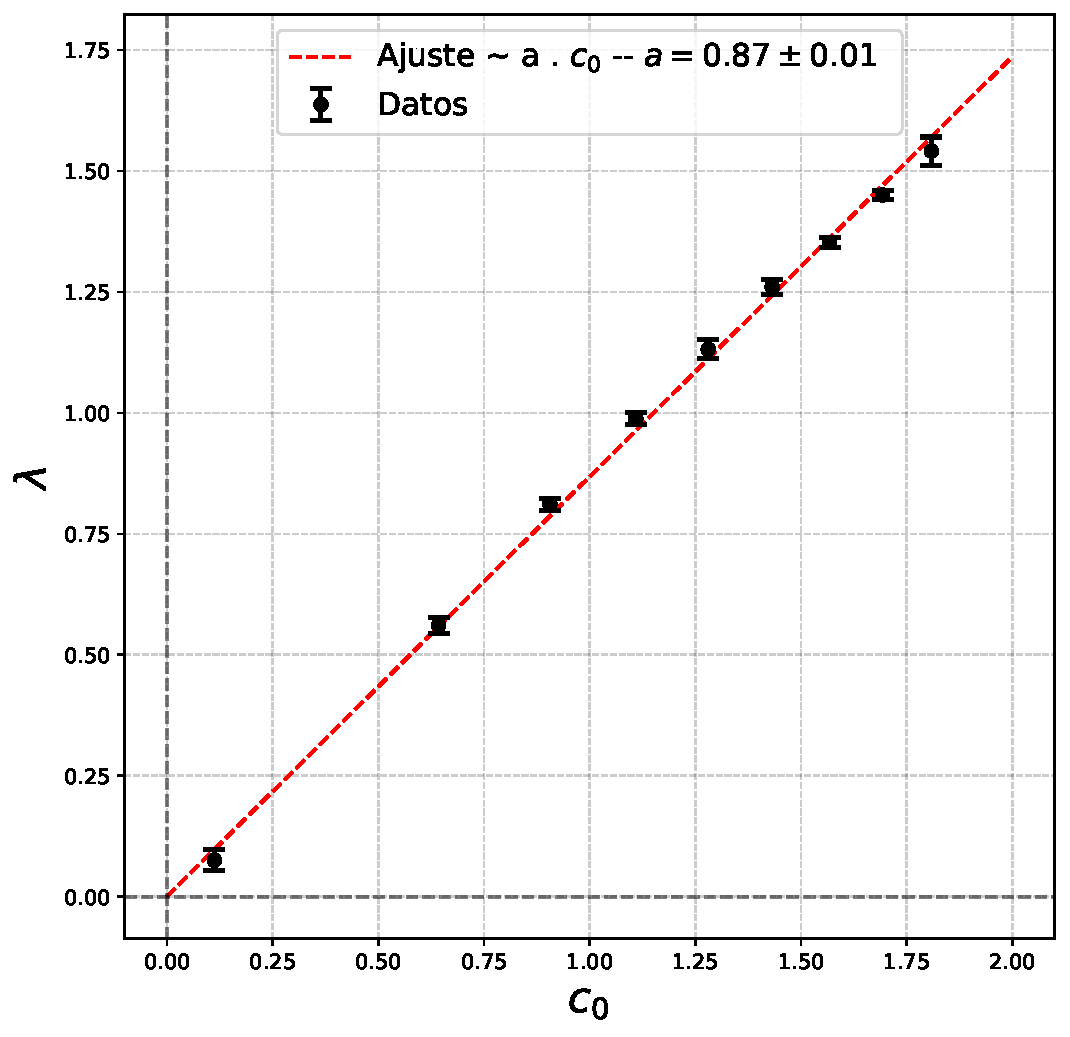
\includegraphics[width=\textwidth]{lambdavsc.pdf}
    \caption{}
\end{subfigure}
    \caption{\textbf{(a)} Velocidad del frente $c$ como función de la inclinación inicial del mismo $m$ para distintos valores de $\beta$. Se observa una dependencia cuadrática. Se utilizó un sistema de $1024\times1024$ con $\gamma = 0.2$, $D_S=0$,$D_I=1$ y $p=0.15$.\textbf{(b)} $\lambda$ como función de la velocidad del frente sin inclinación $c(0)$, se observa que $\lambda\propto c(0)$.}
    \label{fig:tilted_velocity}
\end{figure}

\sect{Factor de estructura}{Sq}

Aquí mostramos la metodología alternativa para determinar los exponentes de universalidad utilizando el factor de estructura $S(q,t)$ dado por 
\begin{equation}
    S(q,t) = \overline{\tilde{u}(q,t)\tilde{u}(-q,t)},
\end{equation}
donde $\tilde{u}(q,t)$ es la transformada de Fourier del campo de desplazamiento $u(y,t)$. Recordamos una vez más del capítulo \ref{cap:intro}, que el factor de estructura con una condición inicial plana para la interfase cumple que,
\begin{equation}
    S(q,t) \propto 
    \begin{cases}
        t^{(1+2\alpha)/z} & \text{si } q \ll \xi_{||}(t)^{-1} \\
        q^{-(1+2\alpha)} & \text{si } q \gg \xi_{||}(t)^{-1}.
    \end{cases}
    \label{abc}
\end{equation}
A partir de estas leyes de potencia podremos determinar los exponentes de universalidad $\alpha$ y $z$. Para empezar, observamos la figura \ref{fig:Sq_t} donde se muestra el factor de estructura $\overline{S(q,t)}$ de la interfase en distintos instantes de tiempo promediado sobre 150 realizaciones y utilizando la definición $u_1(y,t)$ para el campo de desplazamiento. Se utilizó un sistema de tamaño $L_y = 2^{11}\times L_x = 2^{16}$ con $\gamma = 0.2$, $D_S = 0$, $D_I = 1$, $p = 0.15$ y $\beta = 1$. Se observa precisamente el comportamiento descrito por la ecuación \ref{abc}. Es decir, para escalas mayores a la longitud de correlación $\xi_{||}(t)$ el sistema se encuentra descorrelacionado y muestra un espectro de ruido blanco de amplitud creciente con el tiempo, mientras que a distancias menores a $\xi_{||}(t)$ el sistema se encuentra correlacionado y exhibe un espectro de potencias. Cuando la longitud de correlación $\xi_{||}(t)$ alcanza el tamaño del frente $L_y$, el sistema se encuentra completamente correlacionado y queda en un estado estacionario.

\begin{figure}[!t]
    \centering
    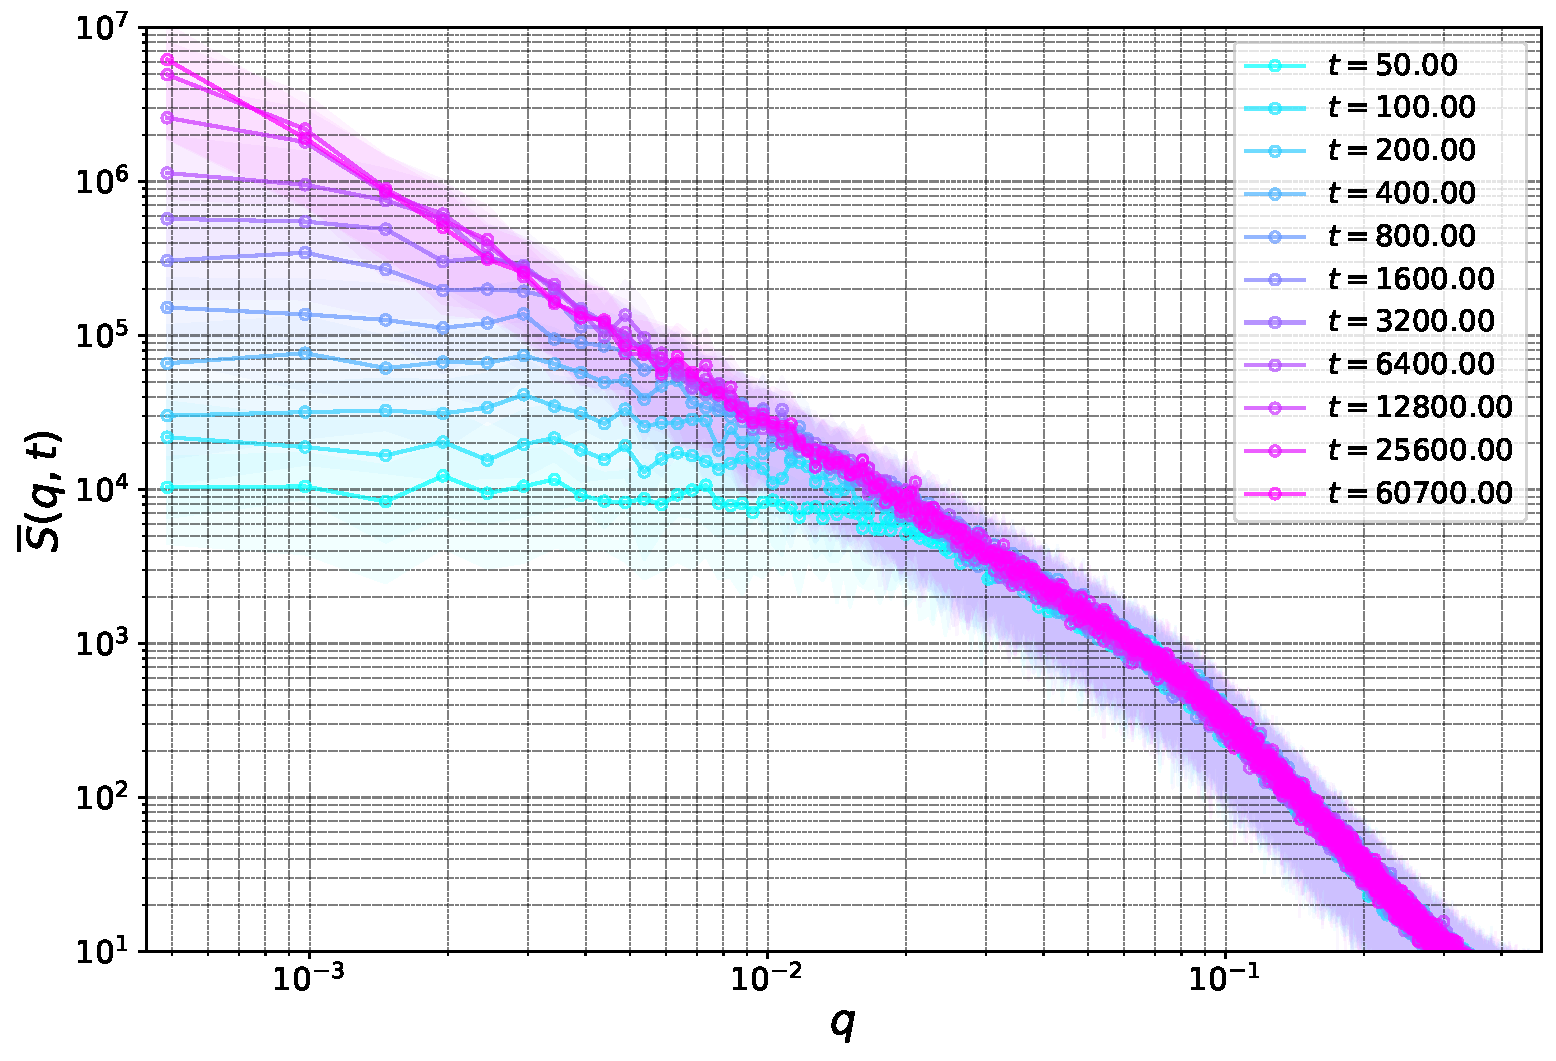
\includegraphics[width=\imsizeL]{Sq_t.pdf}
    \caption{Factor de estructura $\overline{S}(q,t)$ de la interfase en distintos instantes de tiempo promediado sobre 150 realizaciones y utilizando la definición $u_1(y,t)$ para el campo de desplazamiento.. Se utilizó un sistema de tamaño $L_y = 2^{11}\times L_x = 2^{16}$ con $\gamma = 0.2$, $D_S = 0$, $D_I = 1$, $p = 0.15$ y $\beta = 1$. Las sombras de color indican la desviación estándar sobre las realizaciones.}
    \label{fig:Sq_t}
\end{figure}

Para determinar el exponente de rugosidad $\alpha$ definimos el factor de estructura en el estado estacionario, promediando el mismo cuando el tiempo es mayor al tiempo de saturación $t>t_x$, es decir, 
\begin{equation}
    \overline{S}_{est}(q) = \langle \overline{S}(q,t>t_x) \rangle_x.   
\end{equation}
De esta manera aprovechamos el hecho de que el factor de estructura no cambia en el tiempo cuando $t>t_x$ para obtener una medida más precisa del mismo. Los resultados se muestran en la figura \ref{fig:Sq_est_sat}a, utilizando $u_0(y,t)$ y $u_1(y,t)$ y ajustando la ley de potencias $q^{-(1+2\alpha)}$ para grandes escalas ($q<10$) obtenemos $\alpha = 0.40(2)$ con $u_0(y,t)$ y $\alpha = 0.42(2)$ con $u_1(y,t)$. Ambos resultados compatibles entre sí y con los exponentes de rugosidad determinados en la sección \ref{ssec:z_alpha}. Sin embargo, nuevamente quedan por debajo de $\alpha_{KPZ}=\frac{1}{2}$ que predice KPZ. Nuevamente, una razón para la subestimación puede ser que falte tiempo de simulación para alcanzar completamente el estado estacionario.

Nótese también de la figura \ref{fig:Sq_est_sat}a que el factor de estructura proveniente de $u_0(y,t)$ coincide con el dado por $u_1(y,t)$ a grande escalas $q<10$. Sin embargo, para $q>10$ las curvas se separan potencialmente debido nuevamente a que al acercarnos al tamaño de discretización la medición del factor de estructura con $u_0(y,t)$ se ve comprometida.

\begin{figure}[t]
\hspace*{-1.5cm}
\begin{subfigure}{0.55\textwidth}
    \centering
    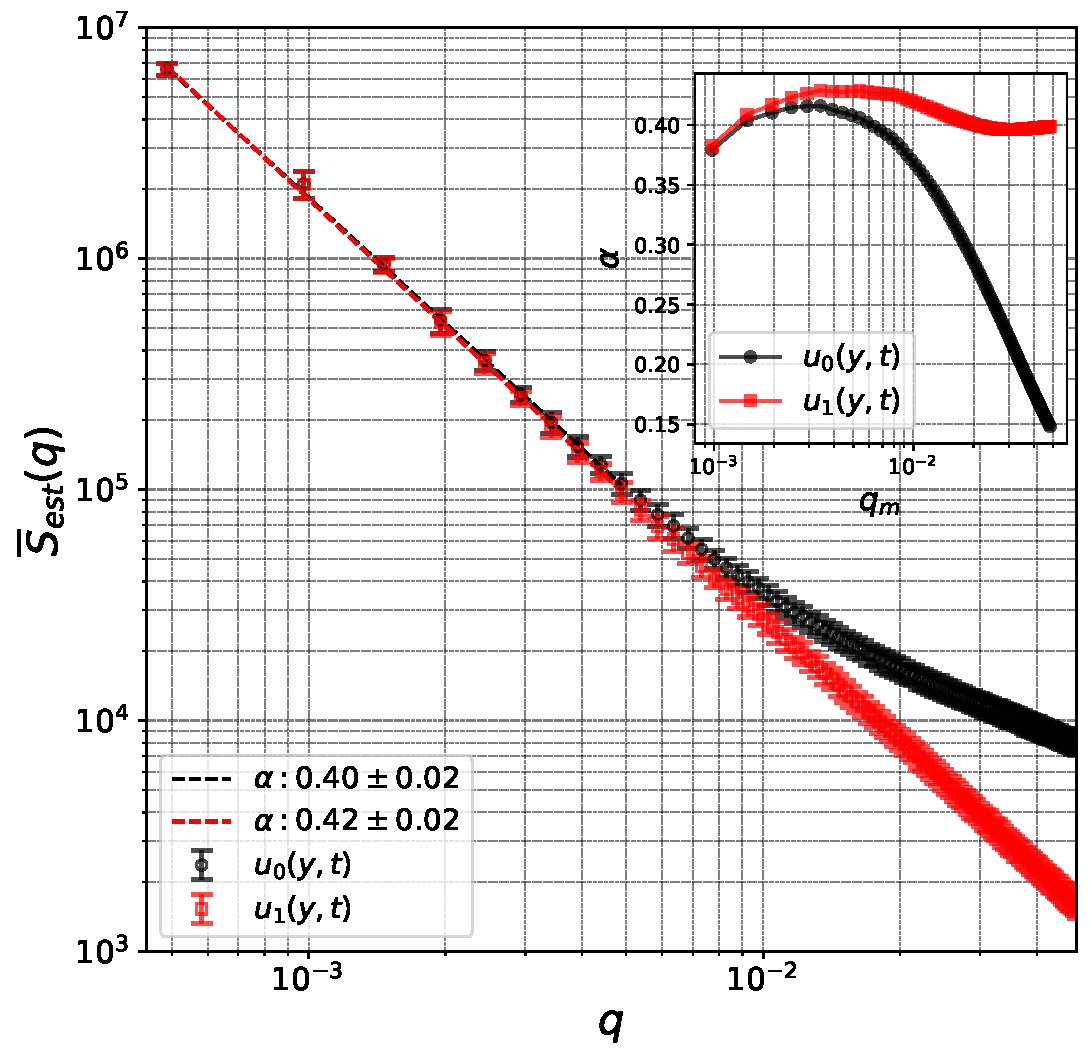
\includegraphics[width=\textwidth]{Sq_est.pdf}
    \caption{}
\end{subfigure}    
\begin{subfigure}{0.55\textwidth}
    \centering
    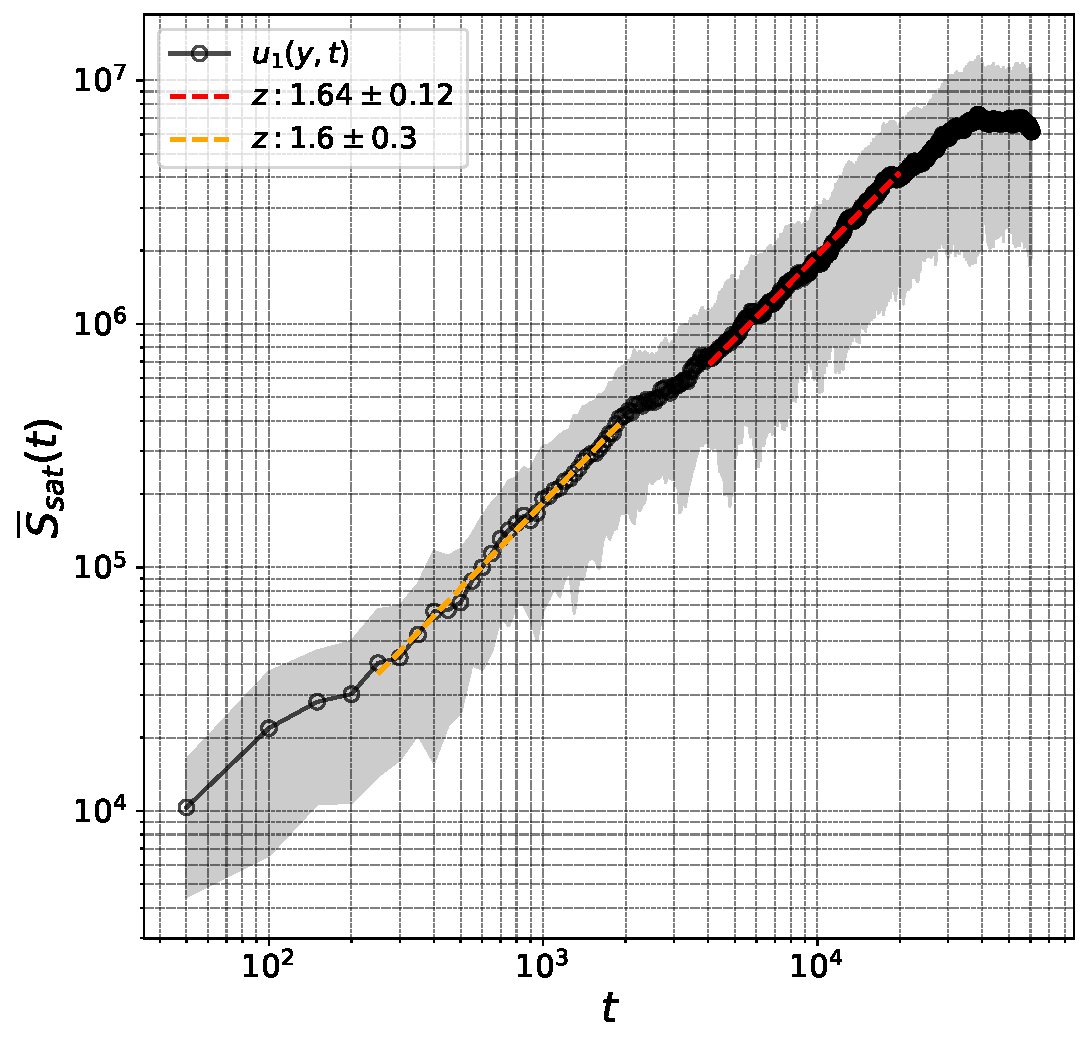
\includegraphics[width=\textwidth]{Sq_sat.pdf}
    \caption{}
\end{subfigure}
    \caption{\textbf{(a)} Factor de estructura en el estado estacionario $\overline{S}_{est}(t)=\langle \overline{S}(q,t>t_x)\rangle_t$ y promediado sobre 150 realizaciones. Se muestra el resultado utilizando $u_0(y,t)$ y $u_1(y,t)$. Se realizó el ajuste dado por la ley de potencia $q^{-(1+2\alpha)}$ para determinar el exponente de rugosidad a grandes escalas ($q\le 10$). En el \textit{inset} se muestra cómo varía el exponente de rugosidad al ajustar la ley de potencias hasta $q_m$. \textbf{(b)} Valor de saturación del factor de estructura en función del tiempo $\overline{S}_sat(t) = \overline{S}(q<\xi^{-1}_{||}(t),t)$ promediado sobre 150 realizaciones. Se muestra solo el resultado con $u_1(y,t)$. Se realizó el ajuste con ley de potencia $t^{(1+2\alpha)/z}$ para determinar el exponente dinámico $z$. Se muestran dos regiones de ajuste porque en el medio se observa un \textit{crossover}.}
    \label{fig:Sq_est_sat}
\end{figure}

Por otro lado, para determinar el exponente dinámico determinamos los valores del factor de estructura en escalas mayores a la longitud de correlación $\xi_{||}(t)$,es decir,
\begin{equation}
    \overline{S}_{sat}(t) = \overline{S}(q<\xi^{-1}_{||}(t),t),
\end{equation}
donde debe cumplirse que
\begin{equation}
    \overline{S}_{sat}(t) \propto t^{(1+2\alpha)/z}.
\end{equation}
Esto es lo que se muestra en la figura \ref{fig:Sq_est_sat}b. Se realizó el ajuste en dos regiones distintas, ya que se observó un \textit{crossovser} en $t\in(2000,3000)$, donde pareciera saturar, pero luego sigue creciendo. Los exponentes dinámicos obtenidos fueron $z = 1.64 \pm 0.12$ y $z = 1.6 \pm 0.2$ que concuerdan con los obtenidos previamente y además son compatibles con el exponente dinámico $z_{KPZ} = \frac{3}{2}$ dado por KPZ.

Finalmente, para verificar visualmente la efectividad de los exponentes obtenidos, en la figura \ref{fig:Sq_colapse} mostramos el colapso del factor de estructura, dividiendo por $t^(1+2\alpha)/z$ y escaleando $q$ por $t^{1/z}$.

\begin{figure}[h]
    \centering
    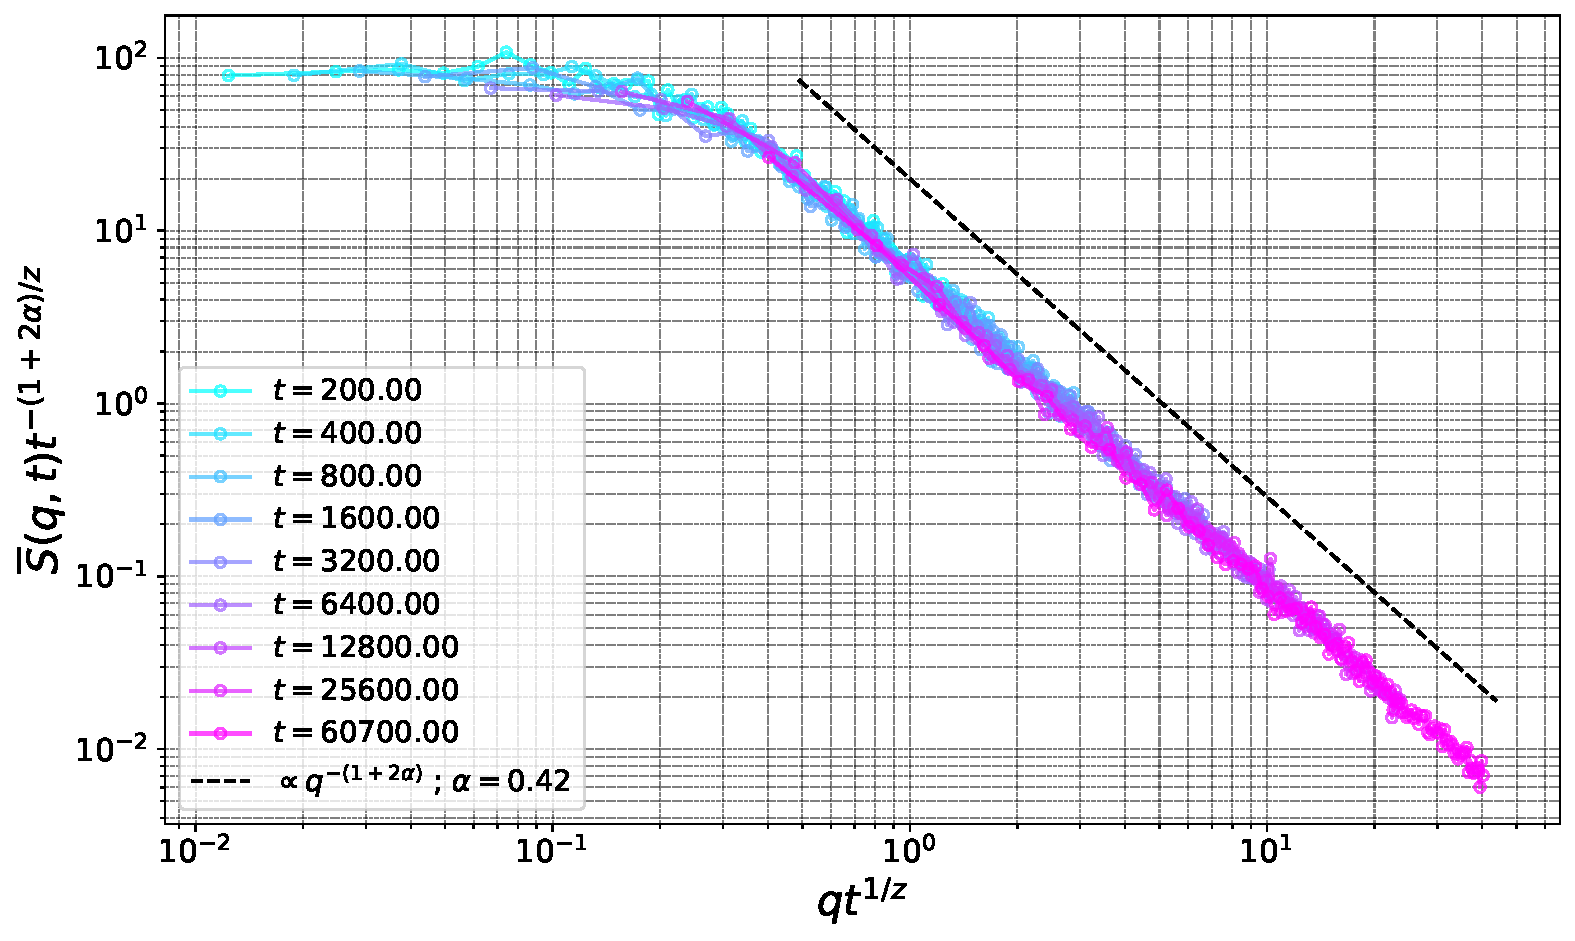
\includegraphics[width=\imsizeL]{Sq_colapse.pdf}
    \caption{Colapso del factor de estructura dado por $u_1(y,t)$ utilizando los exponentes de universalidad $\alpha = 0.42\pm0.02$ y $z = 1.64 \pm 0.12$.}
    \label{fig:Sq_colapse}
\end{figure}

